\documentclass{article}
\usepackage[utf8]{inputenc}
\usepackage[spanish]{babel}
\usepackage[colorlinks]{hyperref}
\usepackage{amsmath}
\usepackage{graphicx}
\usepackage{float}

\begin{document}
\begin{titlepage}
    \centering
    
\includegraphics[width=0.5\textwidth]{images/logo-ugr.png}\par
    \vspace{1cm}
    {\Large\scshape Inteligencia Computacional \par}
    {\huge\bfseries Algoritmos genéticos: \par Problema de la asignación
    cuadrática \par}
    \vspace{0.2cm}
    {\scshape Práctica 2 \par}
    \vfill
    {\large Víctor Vázquez Rodríguez  \par}
    {victorvazrod@correo.ugr.es \par}
    \vfill
    {\large Máster Universitario en Ingeniería Informática \par}
    \vspace{0.2cm}
    {Curso 2019/20 \par}
\end{titlepage}

\tableofcontents\newpage

\section{Introducción}

Hoy en día, el procesamiento de lenguaje natural (NLP por sus siglas en inglés)
es uno de los principales campos de estudio en inteligencia artificial y
\textit{deep learning}. Este campo se centra en la interpretación del lenguaje
humano por parte de ordenadores, permitiendo cosas como el control de
dispositivos con la voz o el análisis y traducción de textos.

Un aspecto muy importante a la hora de procesar y analizar lenguaje natural es
la representación que usamos del mismo, concretamente, cómo representamos las
palabras de forma que un ordenador pueda trabajar con ellas de forma eficiente y
obtener información relevante de su significado y su contexto. Desde el punto de
vista del \textit{machine learning}, podríamos interpretar las palabras de un
texto (o de cualquier conjunto de palabras) como valores de una variable
categórica, donde cada palabra distinta supone una categoría. Uno de los métodos
más comunes y usados para representar este tipo de variables es la codificación
\textit{one-hot}, que nos permite obtener un vector de valores númericos para
cada categoría.

No obstante, esta técnica presenta grandes limitaciones para el procesamiento de
lenguaje natural, de forma que surgen los \textit{word embeddings}. Se trata de
modelos apoyados en las redes neuronales para la proyección o incrustación
(traducción literal de \textit{embedding}) de palabras en un espacio
vectorial~\cite{definition}. En la sección \ref{sec:one-hot-limitations} de este
documento se explican las limitaciones de la codificación \textit{one-hot} y
por qué son necesarios los \textit{word embeddings}, mientras que en la sección
\ref{sec:techniques} se exponen algunas de las técnicas más utilizadas. Al
final, en la sección \ref{sec:example}, se muestra un ejemplo práctico de NLP
con \textit{word embeddings}.
\newpage
\section{Algoritmo base}
La ejecución de un algoritmo genético se compone de varias fases, en cada una de las cuales se pueden aplicar operadores y algoritmos diferentes que, mezclados con los distintos parámetros que se pueden usar, hacen que estos algoritmos sean muy diversos. Al final, todos los algoritmos genéticos siguen la siguiente estructura:

\begin{figure}[H]
\centering
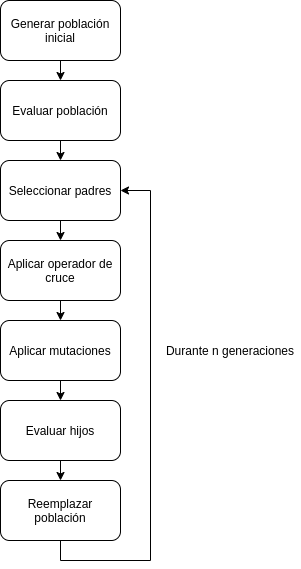
\includegraphics[height=9cm]{images/executionFlow.png}
\end{figure}

Exceptuando la evaluación de los individuos de la población, que se realiza aplicando la función 1 vista en la sección anterior, vamos a ir explicando la implementación escogida para cada una de las partes.

\subsection{Generación de la población inicial}
He decidido usar una población de 100 individuos para el algoritmo, la cuál debe ser inicializada de manera aleatoria. Existen muchas maneras de generar permutaciones aleatorias, de los cuales he decidido aplicar el \textit{Knuth shuffle}. Este algoritmo comienza con una permutación base y va generando nuevas permutaciones cambiando de lugar dos elementos aleatorios de ésta.

\subsection{Selección de los padres}
Del total de la población, debemos elegir un conjunto de individuos para que sean los padres de la nueva generación. Una de las muchas maneras de conseguir esto es mediante torneos, que es el método usado en mi algoritmo. En la selección por torneo, se elige un número $k$ de candidatos aleatorios de la población y se enfrentan unos con otros obteniendo unos ganadores. En mi caso, selecciono 10 candidatos aleatorios de la población inicial y los enfrento de forma determinista para obtener un ganador, es decir, el ganador es el individuo con menor valor de la función de coste.

Repito este procedimiento 100 veces para obtener los 100 padres (los cuales pueden estar repetidos) con los que obtendré los hijos.

\subsection{Cruce de los padres}
Aunque existen muchos operadores de cruce, no todos ellos se pueden aplicar a permutaciones. Los operadores de cruce para representaciones de este tipo deben respetar las restricciones de las mismas. El operador que he aplicado en mi algoritmo es el de cruce de orden, también conocido como \textit{OX}.

Consiste en seleccionar dos índices aleatorios de la permutación que actúa como primer padre y copiar directamente la cadena de elementos que se encuentra entre estos índices a la misma posición en el hijo. A continuación, se rellenan las posiciones que faltan del hijo con los valores del segundo padre que no se encuentran en la cadena copiada, manteniendo el orden de aparición a partir del final de la misma. Dos permutaciones se reparten los roles de primer y segundo padre, obteniendo así 2 hijos.

La probabilidad de cruce es del 100\% lo que significa que todos los padres van a cruzarse. En total, obtenemos 100 nuevos hijos después de cruzar los padres.

\subsection{Mutación de los hijos}
Una vez tenemos los hijos, debemos aplicar un operador de mutación que aporte al algoritmo mayor variabilidad. Cada hijo resultante del cruce de padres tendrá una probabilidad del 80\% de que se le aplique este operador. En mi algoritmo, se usa el intercambio aleatorio como operador de mutación.

Como su propio nombre indica, consiste en seleccionar dos índices aleatorios de la permutación e intercambiar sus elementos de sitio. Los individuos mutados podrán ser mejores o peores que los originales.

\subsection{Reemplazo de la población}
Una vez hemos obtenido y mutado los hijos, debemos incorporar los nuevos individuos a la población actual. Existen varias estrategias para realizar esto (reemplazar la población completa, reemplazar el último elemento, ...), de las que yo he elegido una estrategia elitista.

En el reemplazo elitista, se mantienen los mejores individuos de la generación anterior y se sustituye el resto por los mejores de la nueva generación. En mi caso, me quedo con los 10 mejores individuos y los 90 mejores hijos.\newpage
\section{Variantes baldwiniana y lamarckiana}
Se pueden mejorar los resultados obtenidos por el algoritmo base si se aplica alguna heurística. La idea es que los individuos puedan "aprender", es decir, mejorar sus características. Aplico entonces a mi problema una búsqueda local simple de ascensión de colinas.

El algoritmo de ascensión de colinas se aplica a cada elemento de la población y consiste en ir intercambiando valores de posición para comprobar si se reduce el valor dado por la función de coste. Se podría registrar el nuevo coste de cada uno de los intercambios y quedarse con el mejor, pero esto hace que el algoritmo sea computacionalmente costoso, por lo que sencillamente nos quedamos con el primer intercambio que reduce el coste. Para reducir el tiempo de ejecución del algoritmo, también evitamos recalcular la función de coste tras cada intercambio. En su lugar, calculamos la diferencia en el coste que producen las posiciones afectadas: si la diferencia es negativa, es decir, reduce el coste, aplicamos el intercambio y nos quedamos con el nuevo individuo. De esta forma, obtenemos los mismos resultados en un tiempo muy inferior.

Las variantes baldwiniana y lamarckiana difieren en la capacidad de los hijos para heredar las características aprendidas por los padres, implicando la baldwiniana que no pueden y la lamarckiana que sí. De esta forma, la implementación de estas dos variantes del algoritmo base visto anteriormente consiste en aplicar el algoritmo de ascensión de colinas a la generación actual de individuos en distintas fases del algoritmo genético:

\begin{itemize}
    \item En la variante baldwiniana, se aplica después de haber obtenido los hijos (cruce y mutación) y antes de realizar el reemplazo.
    \item En la variante lamarckiana, se aplica antes de realizar la selección de padres, de forma que los individuos que se cruzan son los mejorados.
\end{itemize}\newpage
\section{Resultados}
Una vez implementados el algoritmo genético y sus dos variantes, lo ejecutamos usando los datos del fichero \textit{tai256c} proporcionado, obteniendo los siguientes resultados:

\begin{table}[H]
\centering
\begin{tabular}{|l|l|l|l|l|}
\hline
Variante & Población & Generaciones & Coste & Tiempo (s) \\ \hline
Base & 100 & 1000 & 45022826 & 3.46 \\ \hline
Baldwiniana & 100 & 150 & 44965852 & 97.36 \\ \hline
Lamarckiana & 100 & 150 & 44920302 & 102.66 \\ \hline
\end{tabular}
\end{table}

Como se puede apreciar, al introducir heurísticas el tiempo de ejecución del algoritmo aumenta considerablemente, pero también obtenemos mejores resultados en un número mucho menor de generaciones que con el algoritmo base, cosa que se puede apreciar mejor en la siguiente gráfica, la cuál muestra la evolución del coste del mejor individuo a lo largo de las generaciones.

\begin{figure}[H]
\centering
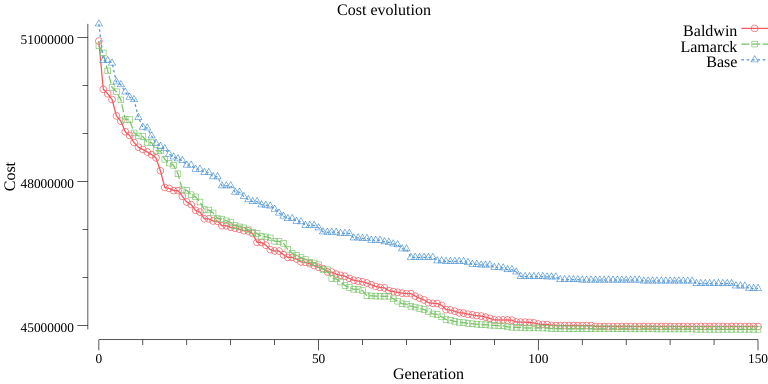
\includegraphics[width=\textwidth]{images/costEvolution.png}
\end{figure}

El mejor resultado lo obtenemos con la variante lamarckiana, aunque su funcionamiento tampoco es mucho mejor que el de la variante baldwiniana, cosa que se puede comprobar en la gráfica.\newpage
\end{document}
